\section{Wpływ zwiększenia budżetu treningowego}
\label{sec:wyniki-budzet-treningowy}

Po zakończeniu podstawowych eksperymentów rozszerzono trening dwóch
konfiguracji wybranych na podstawie wyników walidacyjnych. Dla DQN
była to konfiguracja FEATURES z~nagrodą opartą na zysku netto,
natomiast dla REINFORCE konfiguracja FEATURES ze skalowaną funkcją
nagrody. Dla obu konfiguracji uruchomiono te same ziarna z~budżetem
100\,000 epizodów. Pierwsze 50\,000 epizodów odtworzyło się przy tym
deterministycznie, co sprawdzono, porównując punkty walidacyjne
z~podstawowego przebiegu, więc wynik do 100\,000 epizodów można
traktować jako przedłużenie tej samej trajektorii treningowej.

Przebieg walidacyjnego EV uśredniony po pięciu ziarnach przedstawiono
na rysunku~\ref{fig:extended-learning-curves}. Na osi poziomej
znajduje się liczba epizodów treningowych do 100\,000, a~na osi
pionowej walidacyjne EV, linia pionowa oznacza podstawowy budżet
50\,000 epizodów. Dla DQN wartość końcowa po 100\,000 epizodach jest wyższa niż po
50\,000, mimo lokalnych wahań w~trakcie dalszego treningu. Dla
REINFORCE średnia też rośnie, ale trajektorie poszczególnych ziaren
różnią się od siebie znacznie bardziej.

\begin{figure}[htbp]
    \centering
    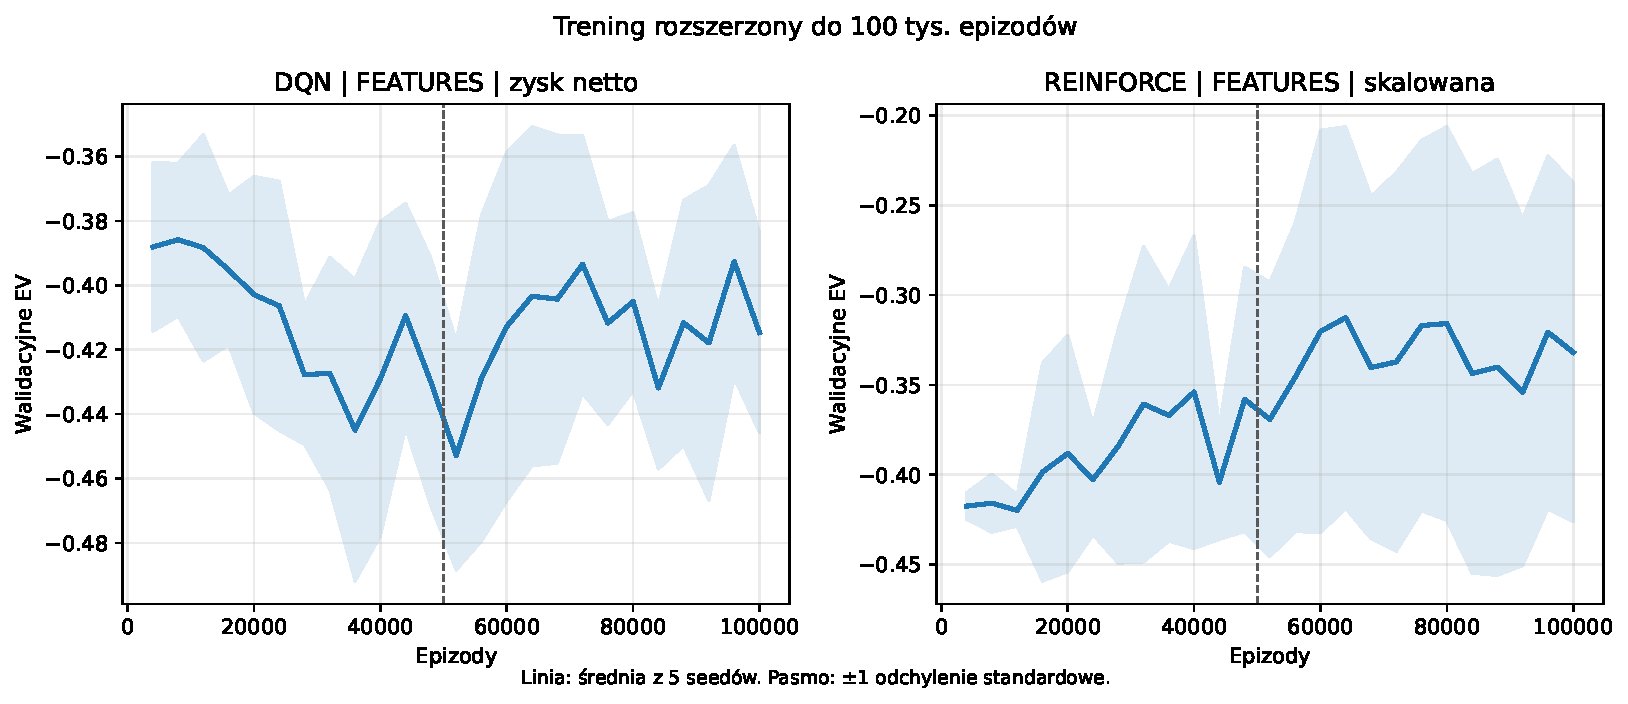
\includegraphics[
        width=\textwidth
    ]{../experiments/results/final_analysis/06_extended_learning_curves.pdf}
    \caption{Przebieg walidacyjnego EV wybranych konfiguracji DQN
    i~REINFORCE do 100\,000 epizodów}
    \label{fig:extended-learning-curves}
\end{figure}

Uśredniona krzywa nie pokazuje jednak, czy poprawa dotyczy wszystkich
ziaren w~podobnym stopniu. Trajektorie poszczególnych przebiegów
przedstawiono na rysunku~\ref{fig:extended-training-per-seed}, z~tymi
samymi osiami co powyżej, dodatkowo z~rozbiciem na pięć kolorów
odpowiadających poszczególnym ziarnom oraz naniesioną krzywą średnią.
Dla REINFORCE widoczna jest też płaska trajektoria odpowiadająca
zdegenerowanym przebiegom. Część linii może się przy tym nakładać,
ponieważ identyczna, deterministyczna polityka oceniana na tym samym
harmonogramie daje identyczny wynik. Jest to zgodne ze zjawiskiem
degeneracji polityki do jednej, niezależnej od stanu akcji, opisanym
szerzej w~sekcji~\ref{sec:wyniki-zachowanie-polityk}.

\begin{figure}[htbp]
    \centering
    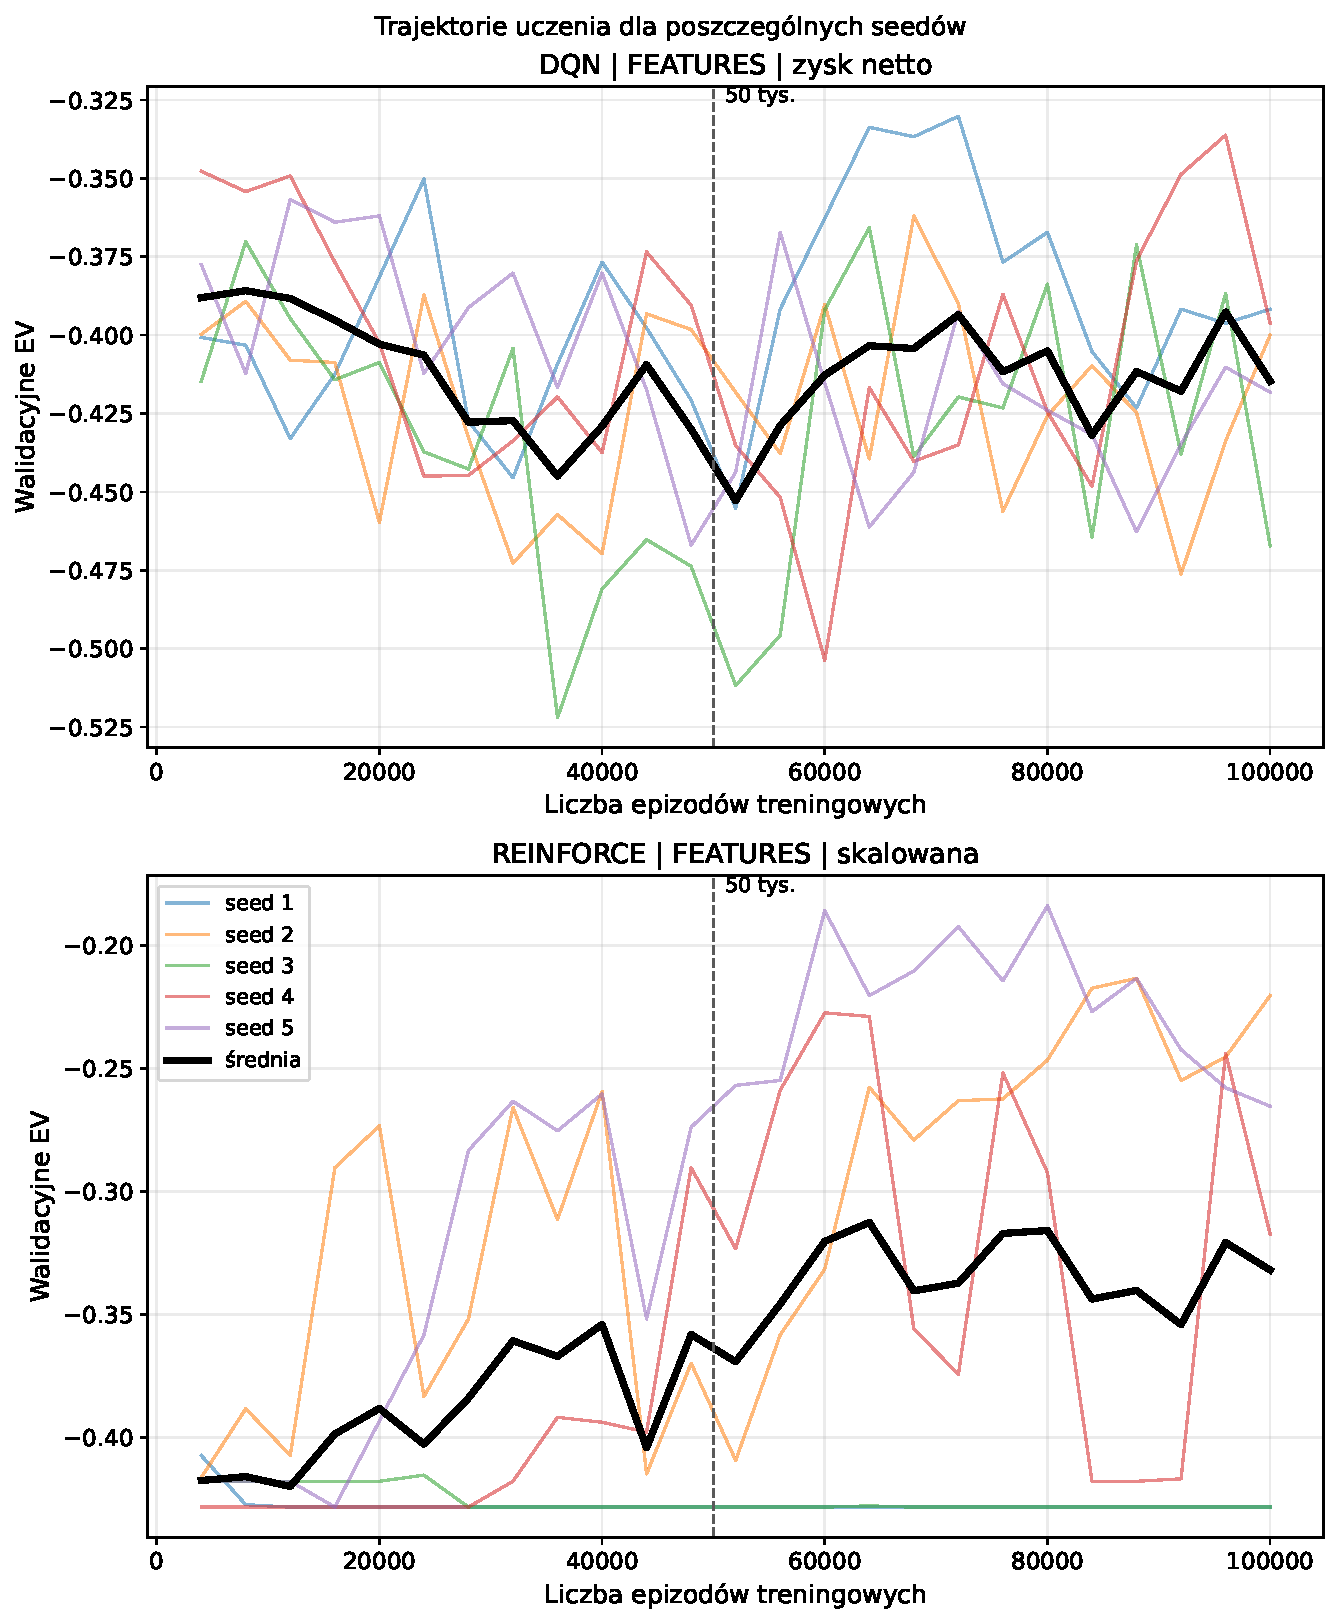
\includegraphics[
        width=0.75\textwidth
    ]{../experiments/results/final_analysis/10_extended_training_per_seed.pdf}
    \caption{Trajektorie walidacyjnego EV dla pięciu ziaren
    wybranych konfiguracji DQN i~REINFORCE}
    \label{fig:extended-training-per-seed}
\end{figure}

Dla DQN wydłużenie treningu prowadziło do stosunkowo spójnej poprawy.
W~końcowej ewaluacji na wspólnych 100\,000 rozdaniach średnie EV
pięciu modeli wzrosło z~$-0{,}4076$ po 50\,000 epizodów do
$-0{,}3859$ po 100\,000 epizodów. Średnia sparowana poprawa wyniosła

\begin{equation}
    \Delta EV_{\mathrm{100k-50k}}
    =
    0{,}0217,
\end{equation}

a~95-procentowy przedział ufności po pięciu ziarnach był równy
$[0{,}0022,\ 0{,}0412]$.

Co istotne, poprawę końcowego EV zaobserwowano dla wszystkich pięciu
ziaren wybranej konfiguracji DQN. Nie oznacza to monotonicznej poprawy na każdym etapie
treningu, co widać na krzywych walidacyjnych, ale rezultat po
100\,000 epizodów był dla każdego ziarna lepszy niż wynik odpowiadającego
mu modelu po 50\,000 epizodów.

Dla REINFORCE średnie EV wzrosło z~$-0{,}3211$ do $-0{,}2943$.
Średnia różnica wyniosła $0{,}0268$, a~więc punktowo była nawet
większa niż dla DQN. Jej 95-procentowy przedział ufności był jednak
równy $[-0{,}0362,\ 0{,}0898]$ i~obejmował zero.

Wynik ten był konsekwencją dużego zróżnicowania zmian pomiędzy
poszczególnymi ziarnami. Niektóre przebiegi REINFORCE poprawiły się
znacznie, podczas gdy inne praktycznie nie zmieniły zachowania lub
uzyskały nieznacznie gorszy wynik. Wydłużenie treningu poprawiło więc
średni rezultat tej konfiguracji, ale nie usunęło problemu
niestabilności procesu uczenia.

Wyniki rozszerzenia budżetu podsumowano w~
tabeli~\ref{tab:extended-training-results}.

\begin{table}[htbp]
    \centering
    \caption{Wpływ zwiększenia budżetu treningowego z~50\,000 do
    100\,000 epizodów dla wybranej konfiguracji FEATURES każdego
    algorytmu}
    \label{tab:extended-training-results}
    \begin{tabular}{lrrrr}
        \toprule
        Algorytm & EV 50k & EV 100k & Różnica & 95\% CI \\
        \midrule
        DQN
            & -0{,}4076
            & -0{,}3859
            & 0{,}0217
            & [0{,}0022,\ 0{,}0412] \\
        REINFORCE
            & -0{,}3211
            & -0{,}2943
            & 0{,}0268
            & [-0{,}0362,\ 0{,}0898] \\
        \bottomrule
    \end{tabular}
\end{table}

Rozszerzony eksperyment jest traktowany jako analiza uzupełniająca.
